\documentclass[unknownkeysallowed]{beamer}
\mode<presentation>
{
%  \usetheme{AnnArbor}
%  \usetheme{Dresden}
%  \usetheme{Montpellier}
%  \usetheme{Antibes}
%  \usetheme{Frankfurt}
%  \usetheme{PaloAlto}
%  \usetheme{Bergen}
%  \usetheme{Boadilla}
%  \usetheme{Goettingen}
%  \usetheme{Pittsburgh}	%!!
%  \usetheme{Berkeley}
%  \usetheme{Hannover}
%  \usetheme{Rochester}		%!!!
%  \usetheme{Berlin}
%  \usetheme{Ilmenau}
%  \usetheme{Singapore}
  \usetheme{Boadilla}		%viel platz
%  \usetheme{JuanLesPins}
%  \usetheme{Szeged}		%!
%  \usetheme{boxes}
%  \usetheme{Luebeck}
%  \usetheme{Warsaw}
%  \usetheme{Copenhagen}
%  \usetheme{Madrid}
%  \usetheme{Darmstadt}
%  \usetheme{Malmoe}
%  \usetheme{default}
%  \usetheme{JuanLesPins}

%  \usetheme{Marburg}


%\usefonttheme{professionalfonts}
%	default | professionalfonts | serif |
%	structurebold | structureitalicserif |
%	structuresmallcapsserif
%\useinnertheme{rounded}
%	circles | default | inmargin |
%	rectangles | rounded

%  \setbeamercovered{transparent}
  % oder auch nicht
\usecolortheme{rose}


\definecolor{uaf yellow}{cmyk}{0,0.16,1,0} % official UAF yellow
\definecolor{light yellow}{cmyk}{0.01,0,0.16,0}
\definecolor{uaf blue}{cmyk}{1,0.66,0,0.02} % official UAF blue
\definecolor{light blue}{cmyk}{0.22,0.11,0,0}
\definecolor{arsc blue}{HTML}{005496}
\definecolor{arsc red}{HTML}{a20a42}
\definecolor{arsc green}{HTML}{009a82}
\definecolor{light gray}{HTML}{777777}

  %navigation aus, klaut nur platz
  \setbeamertemplate{navigation symbols}{}
% Reset title background to default
%\setbeamertemplate{title page}[default]
\setbeamercolor{title}{bg=}
\setbeamercolor{frametitle}{bg=uaf blue, fg=white}
\setbeamercolor{institute}{fg=white}
\setbeamercolor{date}{fg=white}
\setbeamercolor{block}{bg=}
%\setbeamercolor{title}{fg=black}

% Reset block background to default
%\setbeamertemplate{blocks}[default]
%\setbeamercolor{block title}{bg=}
%\setbeamercolor{block body}{bg=}

\beamertemplatenavigationsymbolsempty  
\setbeamertemplate{blocks}[rounded][shadows=false]

\useinnertheme{circles}

}
\usepackage[latin1]{inputenc}
\usepackage{latexsym}
\usepackage{amsfonts}
%\usepackage{natbib}
\usepackage{fancyhdr}
\usepackage{graphicx}
%\usepackage{subfigure}
% oder was auch immer
\usepackage{grffile}
\usepackage{pgf}
\usepackage{tikz}

\usepackage{listings}

\usepackage{times}
\usepackage[T1]{fontenc}
%\usepackage{appendixnumber}
% Oder was auch immer. Zu beachten ist, das Font und Encoding passen
% müssen. Falls T1 nicht funktioniert, kann man versuchen, die Zeile
% mit fontenc zu löschen.

\hypersetup{
    bookmarks=true,         % show bookmarks bar?
    unicode=false,          % non-Latin characters in Acrobat's bookmarks
    pdftoolbar=true,        % show Acrobat's toolbar?
    pdfmenubar=true,        % show Acrobat's menu?
    pdffitwindow=false,     % window fit to page when opened
    pdfstartview={FitH},    % fits the width of the page to the window
    pdftitle={My title},    % title
    pdfauthor={Author},     % author
    pdfsubject={Subject},   % subject of the document
    pdfcreator={Creator},   % creator of the document
    pdfproducer={Producer}, % producer of the document
    pdfkeywords={keyword1} {key2} {key3}, % list of keywords
    pdfnewwindow=true,      % links in new window
    colorlinks=false,       % false: boxed links; true: colored links
    linkcolor=red,          % color of internal links
    citecolor=green,        % color of links to bibliography
    filecolor=magenta,      % color of file links
    urlcolor=cyan           % color of external links
}

\title[PAG]% (optional, nur bei langen Titeln nötig)
{GEOS 436 / 636\\
Programming and Automation for Geoscientists\\[20pt]
-- Week 13: Generic Mapping Tools II --
}

\author[Grapenthin]% (optional, nur bei vielen Autoren)
{Ronni Grapenthin\\
rgrapenthin@alaska.edu\\
Elvey 413B\\
x7682}
% - Namen müssen in derselben Reihenfolge wie im Papier erscheinen.
% - Der \inst{?} Befehl sollte nur verwendet werden, wenn die Autoren
%   unterschiedlichen Instituten angehören.

\institute[UAF] % (optional, aber oft nötig)
{}
% - Der \inst{?} Befehl sollte nur verwendet werden, wenn die Autoren
%   unterschiedlichen Instituten angehören.
% - Keep it simple, niemand interessiert sich für die genau Adresse.

% - Namen müssen in derselben Reihenfolge wie im Papier erscheinen.
% - Der \inst{?} Befehl sollte nur verwendet werden, wenn die Autoren
%   unterschiedlichen Instituten angehören.

% - Der \inst{?} Befehl sollte nur verwendet werden, wenn die Autoren
%   unterschiedlichen Instituten angehören.
% - Keep it simple, niemand interessiert sich für die genau Adresse.

\date[]{}

% - Volle oder abgekürzter Name sind möglich.
% - Dieser Eintrag ist nicht für das Publikum gedacht (das weiß
%   nämlich, bei welcher Konferenz es ist), sondern für Leute, die diese
%   Folien später lesen.

%\AtBeginSection[]
%{
%  \begin{frame}<beamer>
%    \frametitle{Outline}
%    \tableofcontents[currentsection,currentsubsection]
%  \end{frame}
%}

% Falls Aufzählungen immer schrittweise gezeigt werden sollen, kann
% folgendes Kommando benutzt werden:

%\beamerdefaultoverlayspecification{<+->}

%%switch on to have only frame numbers
\setbeamertemplate{footline}[frame number]

\defbeamertemplate*{title page}{customized}[1][]
{
		\begin{tikzpicture}
			\node[text width=\textwidth,
				fill=gray!70, 
				fill opacity=0.75,
				text opacity=1,
				rounded corners = 10pt,
				inner sep=2pt]{
				\begin{center}	
			  \usebeamerfont{title}{\bf \usebeamercolor[fg]{title} \inserttitle}
			  \par
			  \usebeamerfont{subtitle}\insertsubtitle\par
			  \bigskip
			  \usebeamerfont{author}\insertauthor\par
			  \bigskip
			  \usebeamerfont{institute}\insertinstitute\par
			  \bigskip
			  \usebeamerfont{date}\insertdate\par
			  \end{center}
			  };
	\end{tikzpicture}		  
%	\vspace{0.4cm}\usebeamercolor[fg]{titlegraphic}\inserttitlegraphic 
%	\begin{flushright}
%	\vspace{-1.25cm}\includegraphics[width=2cm]{../moore_logo_transp.png}\vspace{5cm}
%	\end{flushright}
}

\begin{document}

\lstset{numbers=left, numberstyle=\tiny, stepnumber=2, basicstyle=\ttfamily, numbersep=5pt, xleftmargin=10pt}

\setbeamertemplate{background}{\includegraphics[width=\paperwidth]{/home/roon/Pictures/rooftop_initial.jpg}}

	\begin{frame}
	\begin{center}
		\titlepage
	\end{center}
	\end{frame}

\setbeamertemplate{background}{}

\begin{frame}
\frametitle{}
%	\vspace{2cm}
	How to automate making publication-quality:

	\begin{itemize}
		\item maps,
		\item x-y plots, 
		\item animations 
	\end{itemize}

	using world class base data sets while having maximum flexibility regarding layout of your product?
\end{frame}


\begin{frame}
\frametitle{}
	\begin{center}
		
\includegraphics[width=.8\textwidth]{../figures/gmt-logo.png}	
	\end{center}
	\begin{flushright}
	\tiny{\emph{\url{https://www.generic-mapping-tools.org}}}
	\end{flushright}	
\end{frame}

\begin{frame}[fragile=singleslide]
\frametitle{Changing {\tt gmtdefaults}}
	Last time:
\begin{verbatim}
	gmt set MAP_FRAME_TYPE plain
\end{verbatim}		
	What other parameters are there?
\end{frame}


\begin{frame}
\frametitle{Changing {\tt gmtdefaults}}
	\begin{center}
		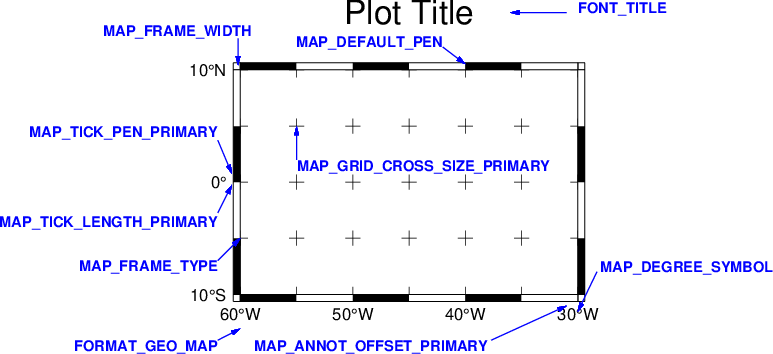
\includegraphics[width=\textwidth]{../figures/gmt_defaults_1a.png}	
	\end{center}
	\begin{flushright}
	\tiny{\emph{\url{https://www.generic-mapping-tools.org}}}
	\end{flushright}	
\end{frame}

\begin{frame}
\frametitle{Changing {\tt gmtdefaults}}
	\begin{center}
		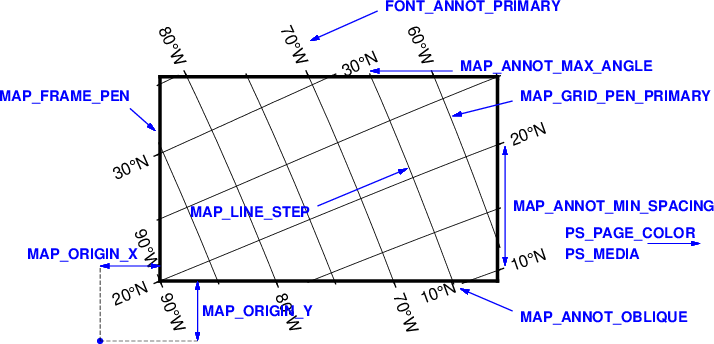
\includegraphics[width=\textwidth]{../figures/gmt_defaults_1b.png}	
	\end{center}
	\begin{flushright}
	\tiny{\emph{\url{https://www.generic-mapping-tools.org}}}
	\end{flushright}	
\end{frame}

\begin{frame}[fragile=singleslide]
\frametitle{Changing {\tt gmtdefaults}}
Basic Syntax:
\begin{verbatim}
gmt set PARAMETER1 value1 PARAMETER2 value2 ...
\end{verbatim}		
	\begin{itemize}
		\item Use in shell script or on command line
		\item Changes defaults temporarily (session)
		\item Can be called many times
		\item Can be called to set values for a few commands and then reset them later.
		\item See \url{https://docs.generic-mapping-tools.org/latest/gmt.conf.html} for full list or parameters.
	\end{itemize}
\end{frame}

\begin{frame}[fragile=singleslide]
\frametitle{Changing {\tt gmtdefaults}}
Another example
{\scriptsize
\begin{verbatim}
gmt set FONT_ANNOT_PRIMARY 12p,Helvetica MAP_GRID_CROSS_SIZE_PRIMARY 0.1i 
\end{verbatim}		
}
\end{frame}

\begin{frame}
\frametitle{Grids}
	\begin{itemize}
		\item We used GMT's mechanism to download a topo grid for Mt. St. Helens 
		\item Downloaded to netCDF files (for 1\,s resolution) in {\scriptsize {\tt $\sim$/.gmt/server/earth/earth\_relief/earth\_relief\_01s\_g/}}
		\item netCDF is special format to combine data and meta data
		\item We can inspect this with {\tt gmt grdinfo}
	\end{itemize}
\end{frame}

\begin{frame}[fragile=singleslide]
\frametitle{Grids}
\begin{verbatim}
gmt grdinfo N46W122.earth_relief_01s_g.nc
\end{verbatim}
	\begin{center}
		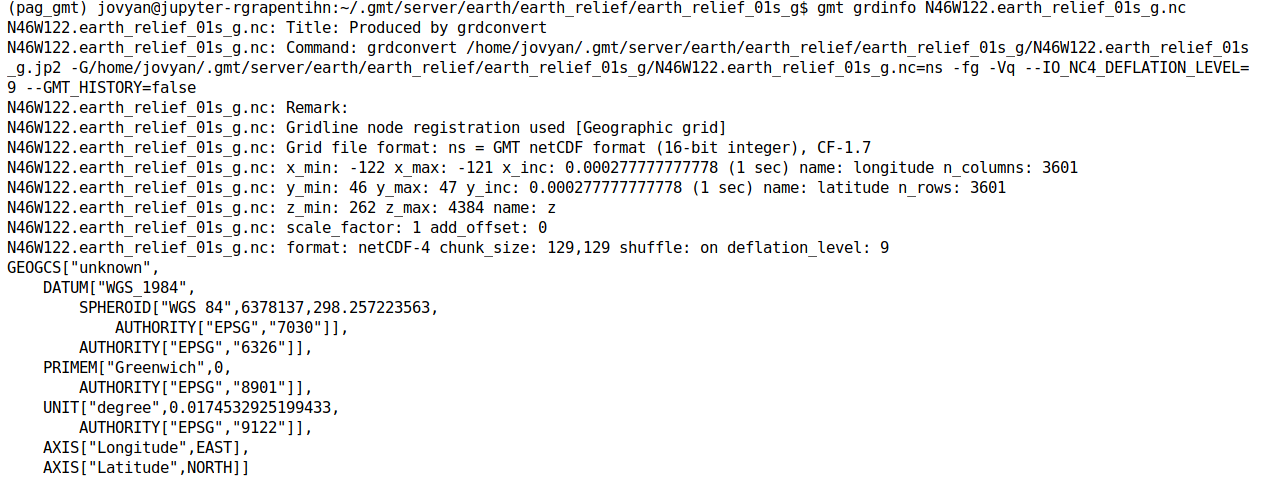
\includegraphics[width=\textwidth]{../figures/gmt_grdinfo_example.png}	
	\end{center}

\end{frame}

\begin{frame}
\frametitle{Why have data on grids?}
	\begin{itemize}
		\item Provides regular spacing
		\item Easy to contour
		\item Easy quantitative analysis
		\item Consistent representation of data
		\item Saves disk space (store two coordinates, x and y increments, and data values)
	\end{itemize}
\end{frame}

\begin{frame}
\frametitle{Contouring gridded data sets}
\begin{itemize}
\item Use {\tt grdcontour} on {\tt .grd, .nc} files
\item Produces contour map by tracing each contour through 2D grid
\item Could also save x,y,z positions of contour lines to output files
\item \dots has many options, most useful ones:
\end{itemize}
	\begin{center}
		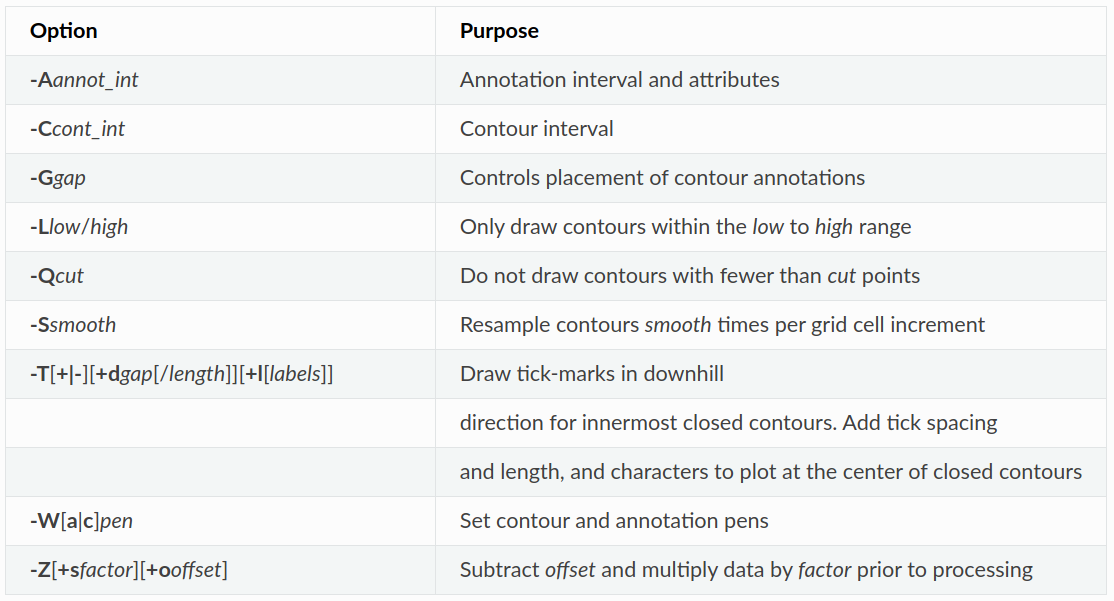
\includegraphics[width=.9\textwidth]{../figures/gmt_grdcontour.png}	
	\end{center}
	\vspace{-0.5cm}
	\begin{flushright}
	\tiny{\emph{\url{https://www.generic-mapping-tools.org}}}
	\end{flushright}	
\end{frame}


\begin{frame}[fragile=singleslide]
\frametitle{Contouring Mt. St. Helens example}
{\scriptsize
\begin{verbatim}
#grdcut the region of interest from earth relief data set
gmt grdcut @earth_relief_01s -R-122.4/-121.95/46.0/46.33 -Gsthelens.nc -V
\end{verbatim}
}
\begin{center}
	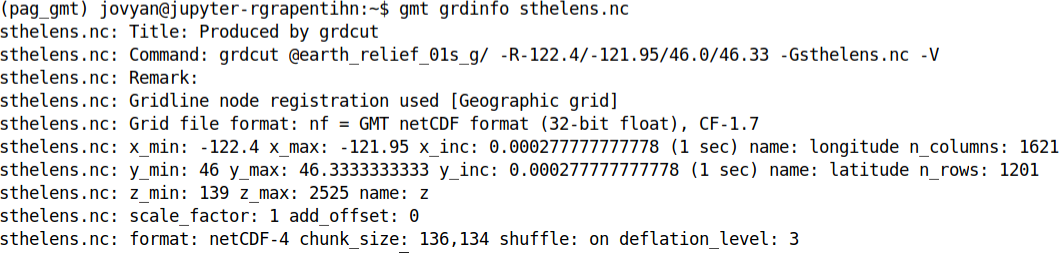
\includegraphics[width=\textwidth]{../figures/gmt_grdcut_sthelens.png}	
\end{center}
\end{frame}

\begin{frame}[fragile=singleslide]
\frametitle{Contouring Mt. St. Helens example}
{\scriptsize
\begin{verbatim}
#grdcut the region of interest from earth relief data set
gmt grdcontour sthelens.nc -JM6i -C100 -A500 -B -png sthelens_contour
\end{verbatim}
}
{\scriptsize
\begin{verbatim}
#can also use earth_relief directly
gmt grdcontour @earth_relief_01s -R-122.4/-121.95/46.0/46.33 -JM6i -C100 -A500 -B -png sthelens_contour
\end{verbatim}
}

\end{frame}

\begin{frame}[fragile=singleslide]
\frametitle{Contouring Mt. St. Helens example}
\begin{center}
	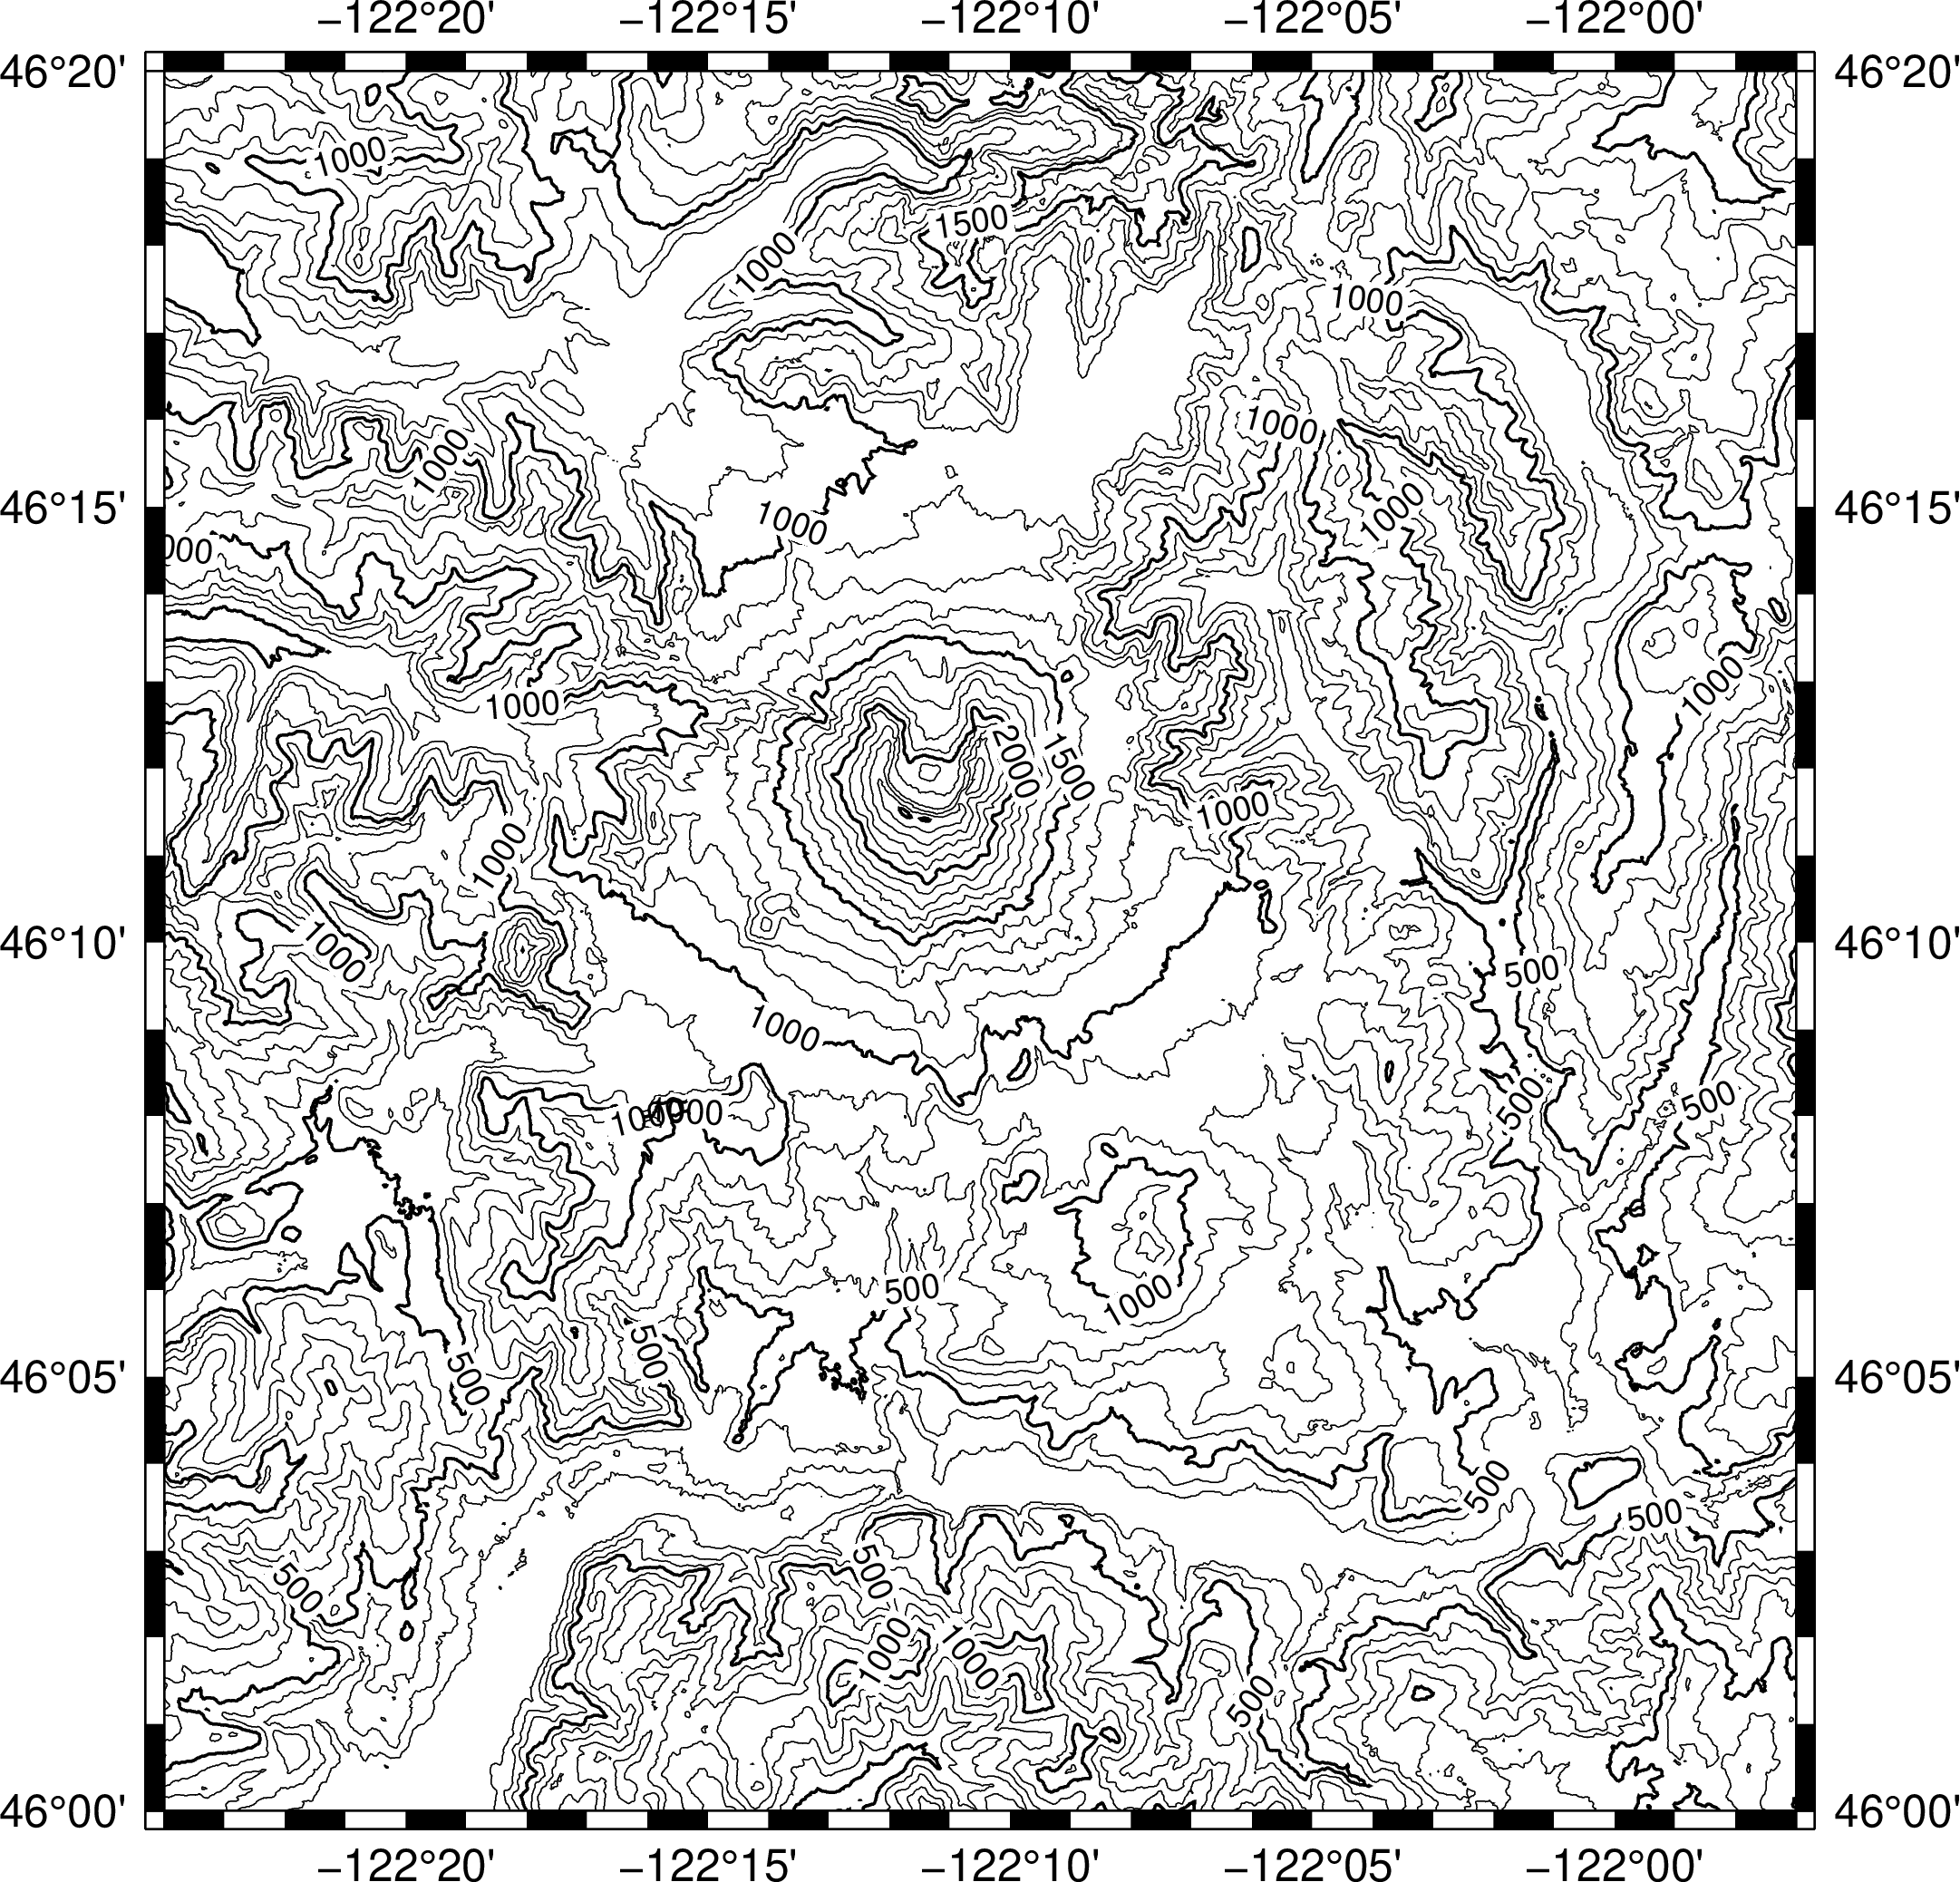
\includegraphics[width=.7\textwidth]{../figures/gmt_sthelens_contours.png}	
\end{center}
\end{frame}

\begin{frame}[fragile=singleslide]
\frametitle{Don't have a {\tt .grd} file \dots}
Use {\tt xyz2grd}
	\begin{itemize}
		\item Converts z-table or xyz-table to regular grid file
		\item Reports if nodes are lacking data
		\item Fills such nodes with user-specified value or NaN
		\item Nodes with multiple values will be set to mean
		\item Does {\bf not} grid the data, just reformat!
	\end{itemize}
\end{frame}


\begin{frame}[fragile=singleslide]
\frametitle{Gridding of arbitrarily spaced data}
	\begin{itemize}
		\item Requires interpolation onto regular grid (called ``gridding'')
		\item All gridding modules in GMT must specify gridding domain (region, increment; -R, -I) and output grid filename (-G)
	\end{itemize}
\end{frame}

\begin{frame}[fragile=singleslide]
\frametitle{Nearest Neighbor Gridding: {\tt nearneighbor}}
	\begin{columns}[t]
	\column{.5\textwidth}
		\begin{itemize}
			\item Preferred for high data density
			\item Simple nearest neighbor averaging, weighted by distance from node
			\item Local procedure: only considers data inside search radius (-S) around output grid node
		\end{itemize}
	\column{.5\textwidth}
		\begin{center}
			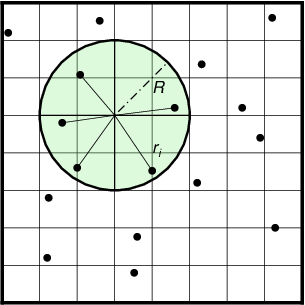
\includegraphics[width=.9\textwidth]{../figures/gmt_nearneighbor.png}	
		\end{center}
		\vspace{-0.5cm}
		\begin{flushright}
		\tiny{\emph{\url{https://www.generic-mapping-tools.org}}}
		\end{flushright}	
	\end{columns}
\end{frame}

\begin{frame}[fragile=singleslide]
\frametitle{Other gridding methods}
	\begin{itemize}
		\item {\tt surface} - Splines in tension: global procedure; try to force thin elastic plate to go through all data points
		\item {\tt sphinterpolate} - Spherical gridding in tension of data on a sphere
		\item {\tt triangulate} - Delaunay triangulation or Voronoi partitioning and gridding of Cartesian data
	\end{itemize}
\end{frame}

\begin{frame}[fragile=singleslide]
\frametitle{Adding Color {\tt grdimage}}
	various options to get a pallete to use with {\tt -C}
	\begin{itemize}
		\item use built-in color palette name with {\tt -C}, see \url{https://docs.generic-mapping-tools.org/latest/cookbook/cpts.html#of-colors-and-color-legends} automatically scaled to grid's z-range
		\item use {\tt makecpt} to generate color palette table (saved to session default cpt), can set transparency, 
			\begin{itemize}
				\item Make cpt with values from -200 to 200 with discrete color change every 25; use polar blue-white-red colortable
				\item {\scriptsize {\tt gmt makecpt -Cpolar -T-200/200/25 > colors.cpt}}
			\end{itemize}
		\item use {\tt grd2cpt} to make color palette table from one or more grids (e.g., when desired symmetric around zero use {\tt -Sh|l|m|u}
		\item {\tt -A} flag enables transparency
	\end{itemize}	
\end{frame}


\begin{frame}[fragile=singleslide]
\frametitle{Mt. St. Helens {\tt gridimage}}
		\begin{center}
			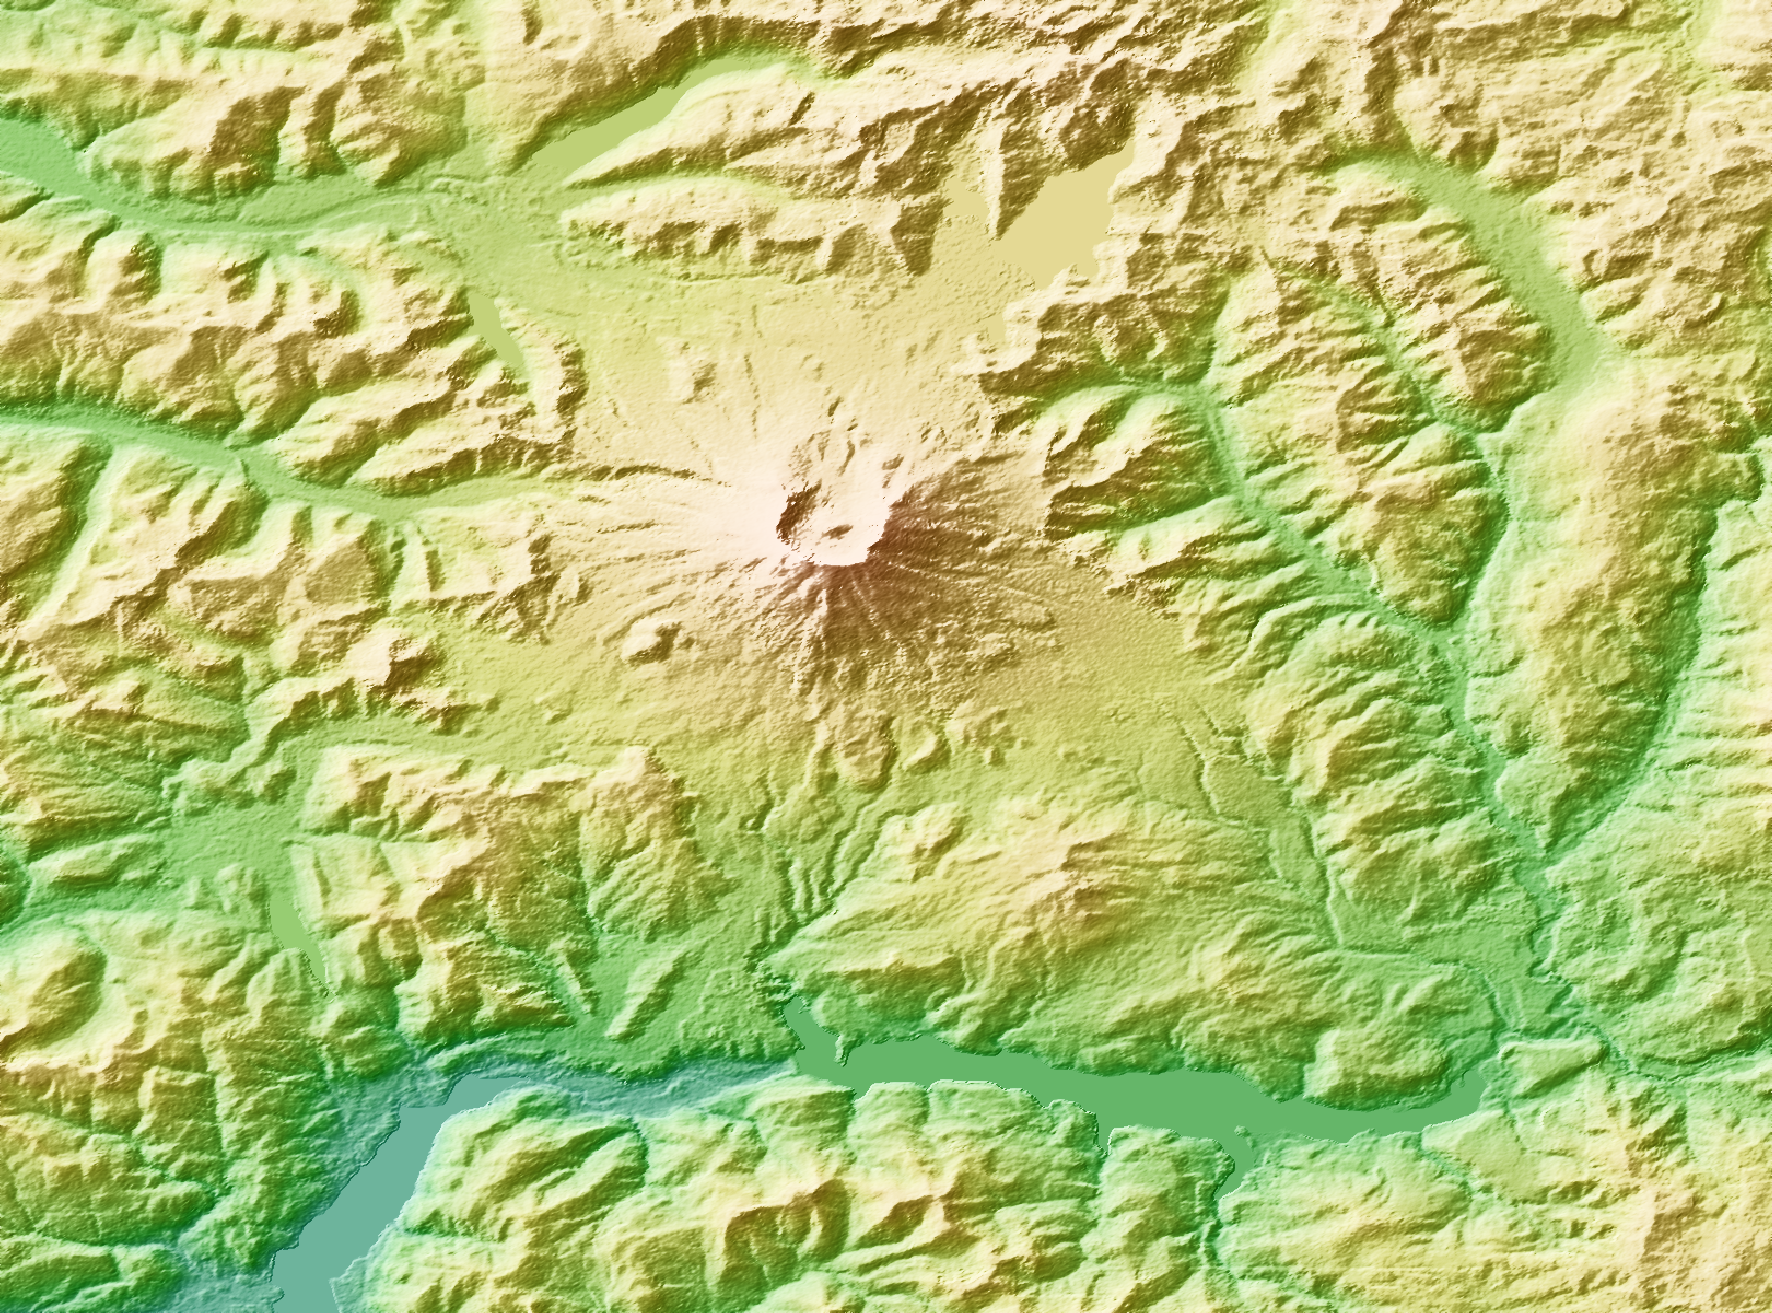
\includegraphics[width=.7\textwidth]{../figures/gmt_sthelens_grid.png}	
		\end{center}
{\scriptsize
	\begin{verbatim}
gmt makecpt -T0/5000/10 -Z -Ctopo > sthelens.cpt
gmt grdimage sthelens.nc -Csthelens.cpt -png sthelens_grid -I
	\end{verbatim}
}
\end{frame}

\begin{frame}[fragile=singleslide]
\frametitle{Mt. St. Helens {\tt gridimage}}
		\begin{center}
			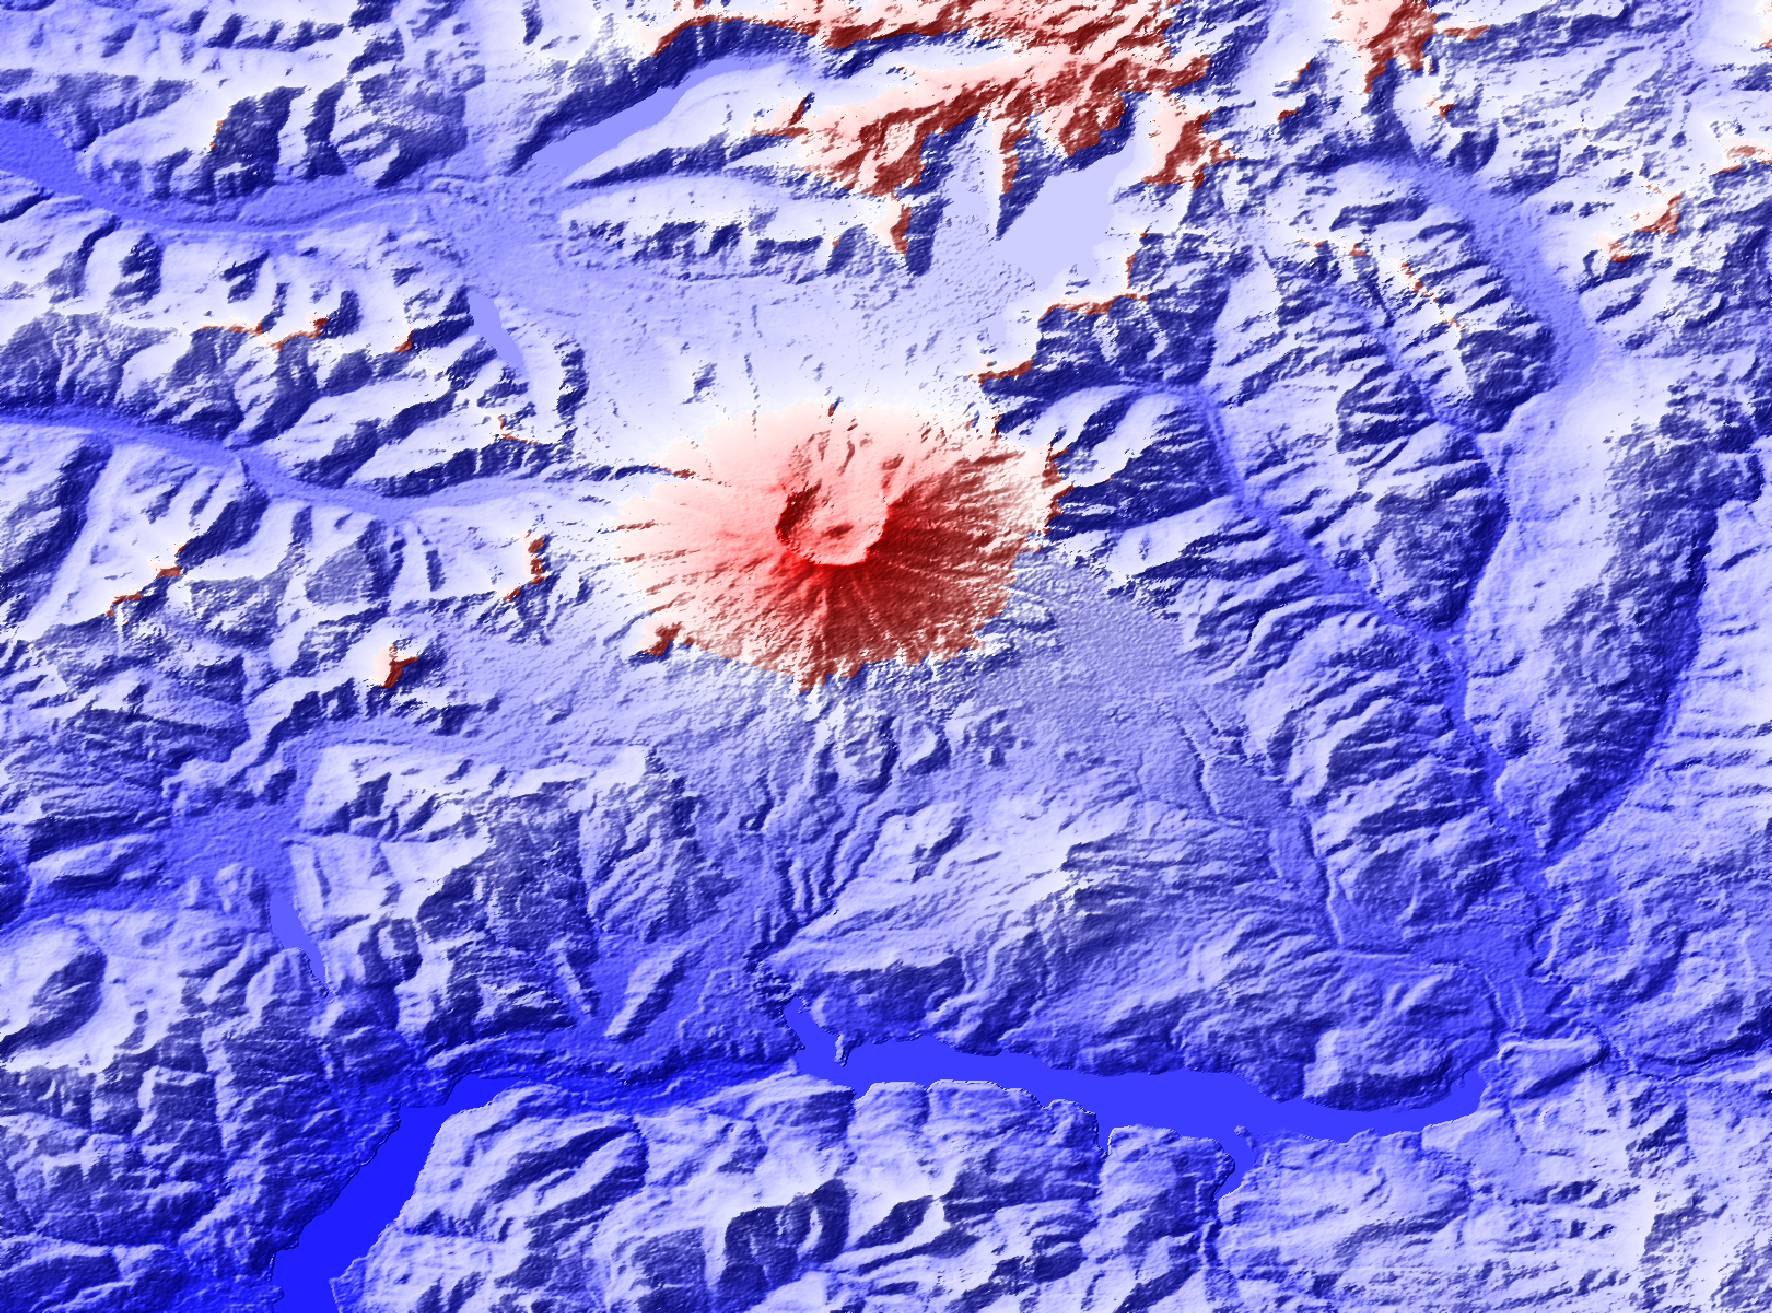
\includegraphics[width=.7\textwidth]{../figures/gmt_sthelens_grid_polar.png}	
		\end{center}
{\scriptsize
	\begin{verbatim}
gmt makecpt -T0/2600/10 -Z -Cpolar > sthelens.cpt
gmt grdimage sthelens.nc -Csthelens.cpt -png sthelens_grid -I
	\end{verbatim}
}
(color palettes can be misleading)
\end{frame}


\begin{frame}[fragile=singleslide]
\frametitle{Grid Operations}
	\begin{center}
		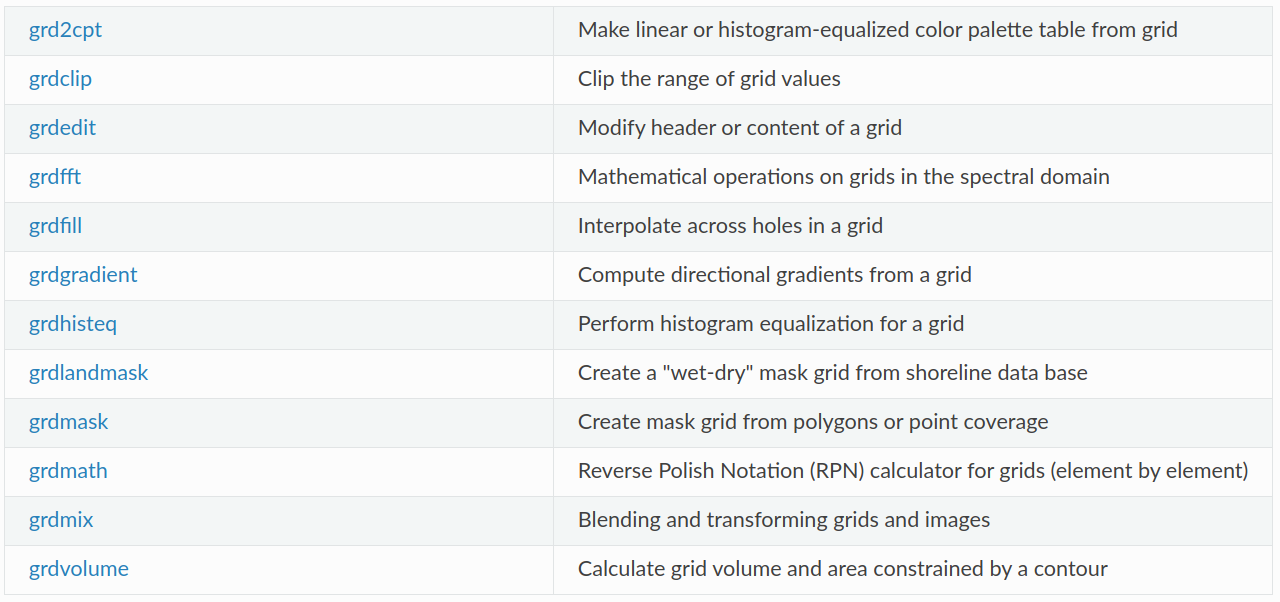
\includegraphics[width=\textwidth]{../figures/gmt_grd_ops.png}	
	\end{center}
	\vspace{-0.5cm}
	\begin{flushright}
	\tiny{\emph{\url{https://www.generic-mapping-tools.org}}}
	\end{flushright}	
\end{frame}

\begin{frame}[fragile=singleslide]
\frametitle{For Ternary Enthusiasts}
	\begin{center}
		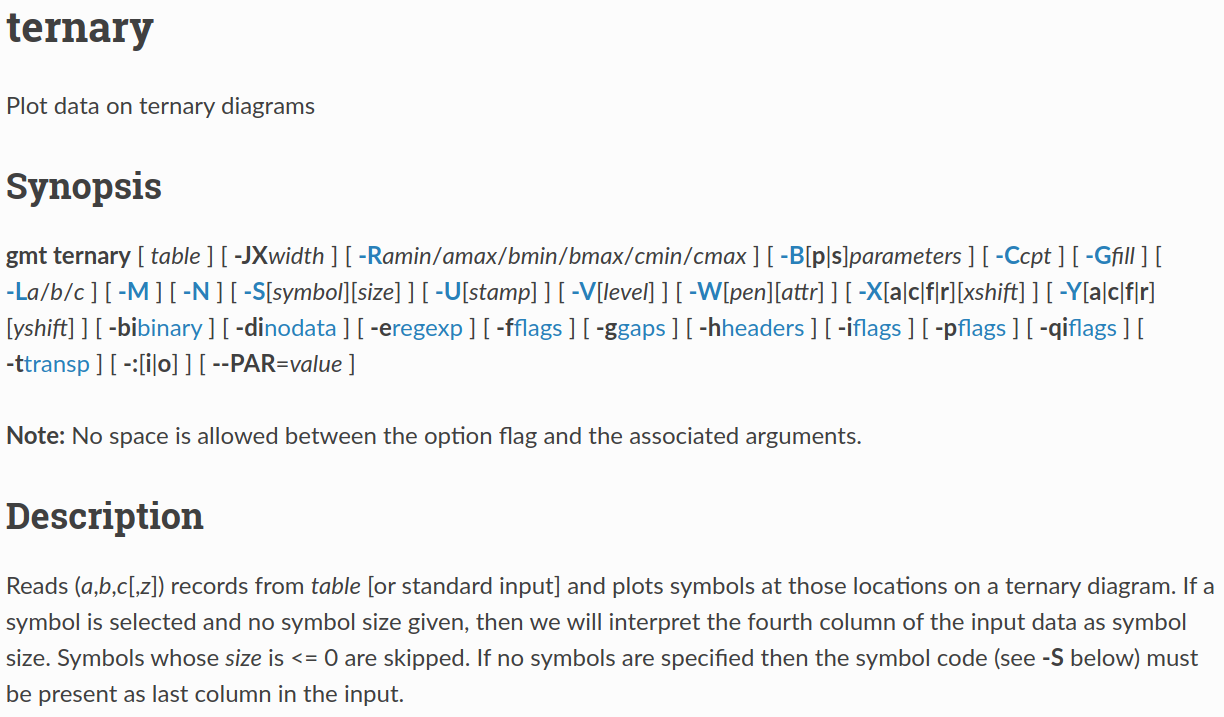
\includegraphics[width=.9\textwidth]{../figures/gmt_ternary.png}	
	\end{center}
	\vspace{-0.5cm}
	\begin{flushright}
	\tiny{\emph{\url{https://www.generic-mapping-tools.org}}}
	\end{flushright}	
\end{frame}

\begin{frame}[fragile=singleslide]
\frametitle{For Ternary Enthusiasts}
{\scriptsize
	\begin{verbatim}
gmt begin ternary_map png
gmt makecpt -Cturbo -T0/80/10
gmt ternary @ternary.txt -R0/100/0/100/0/100 -JX6i \
    -Sc0.1c -C -LWater/Air/Limestone \
    -Baafg+l"Water component"+u" %" \
    -Bbafg+l"Air component"+u" %" \
    -Bcagf+l"Limestone component"+u" %" \
    -B+givory+t"Example data from MATLAB Central"
gmt end
	\end{verbatim}	
}
	\begin{flushright}
	\tiny{\emph{\url{https://www.generic-mapping-tools.org}}}
	\end{flushright}	
\end{frame}

\begin{frame}
\frametitle{}
	\begin{center}
		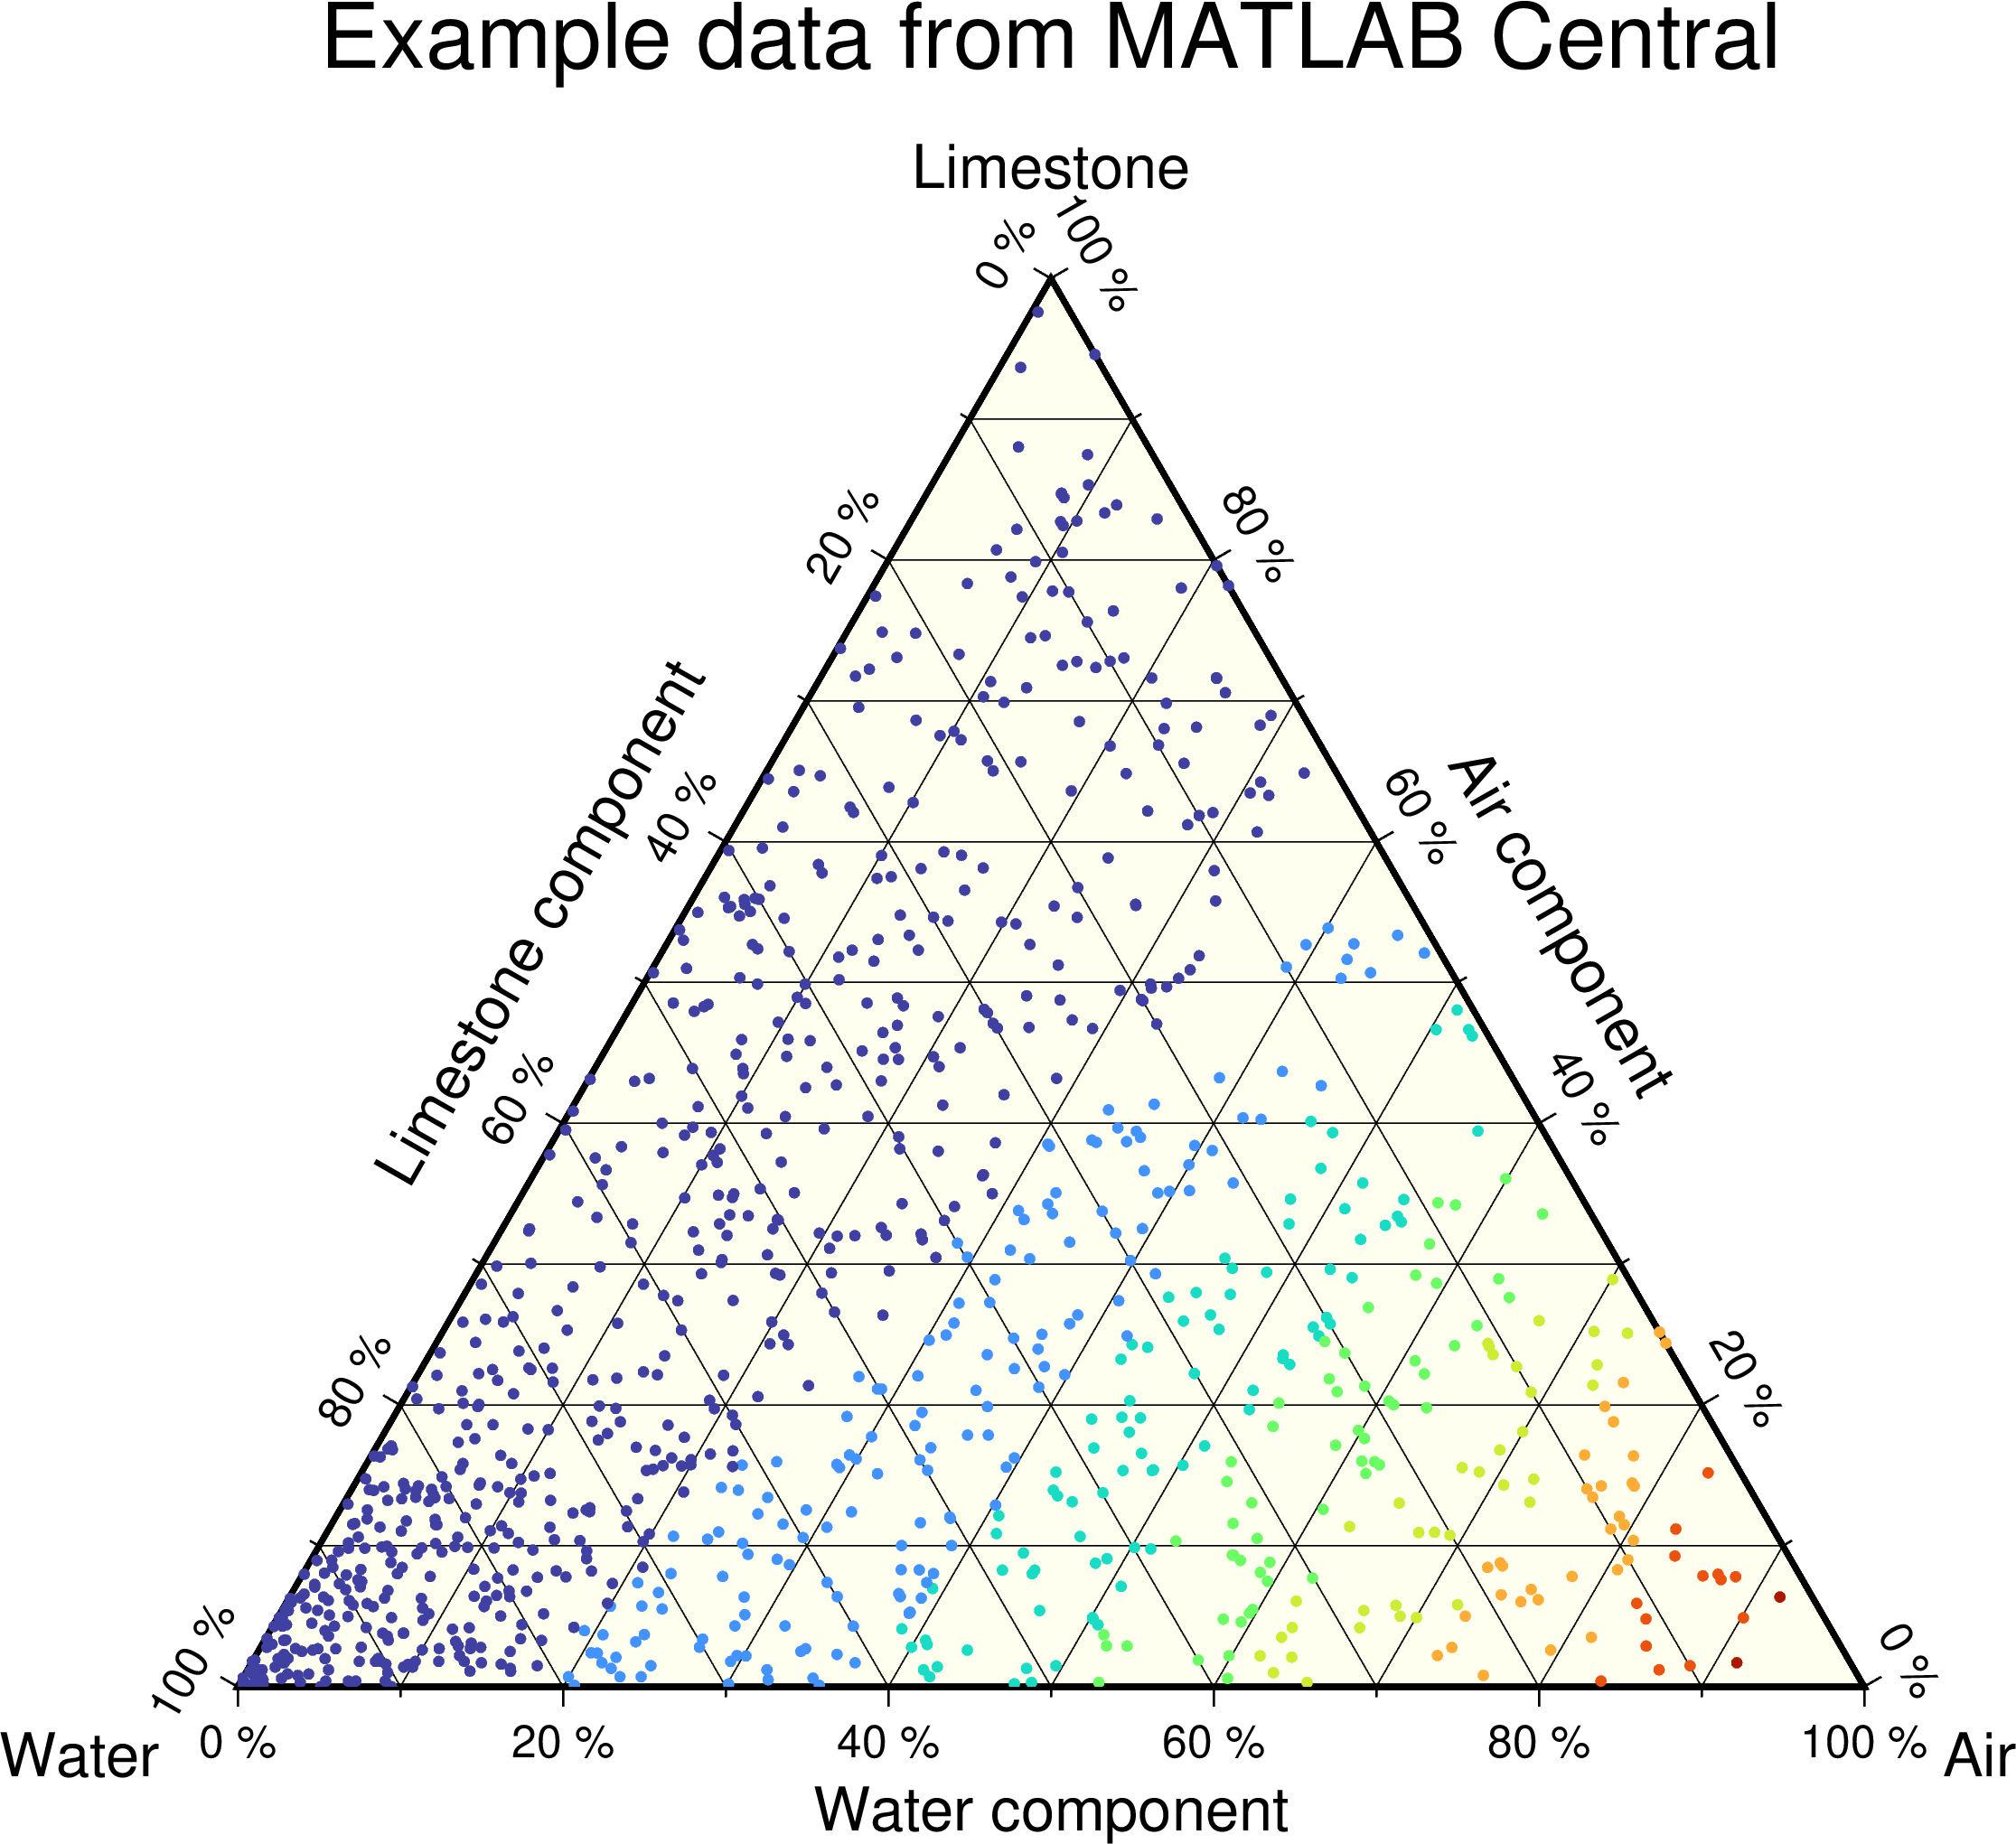
\includegraphics[width=.8\textwidth]{../figures/gmt_ternary_map.png}	
	\end{center}
	\vspace{-0.35cm}
	\begin{flushright}
	\tiny{\emph{\url{https://www.generic-mapping-tools.org}}}
	\end{flushright}	
\end{frame}

\begin{frame}
\frametitle{\dots so much more}
	\begin{center}
		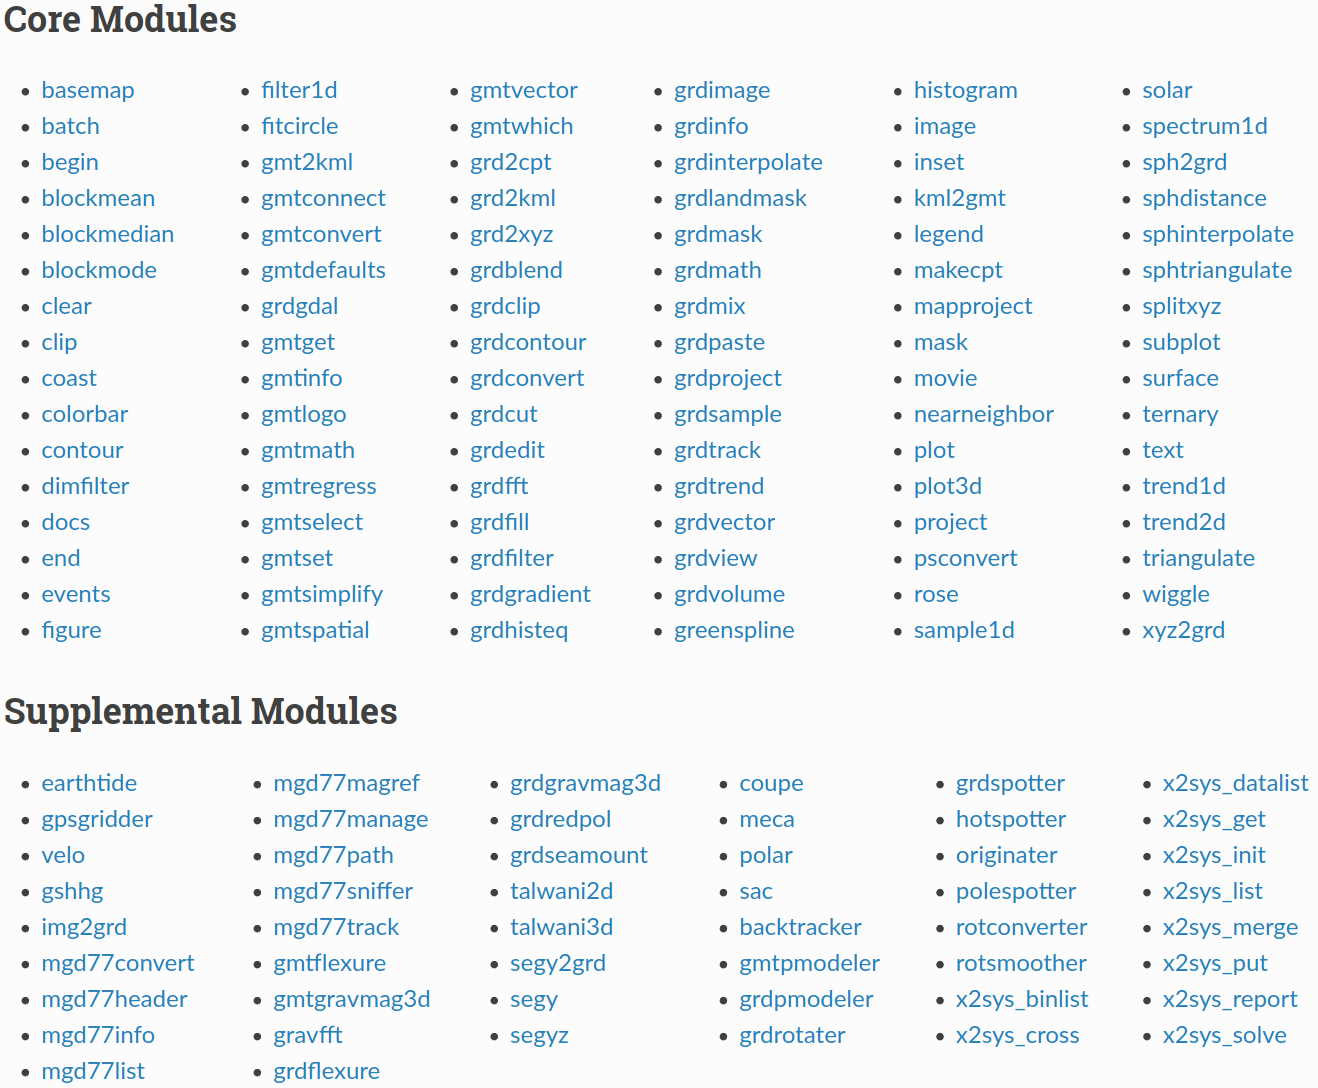
\includegraphics[width=.8\textwidth]{../figures/gmt_modules.png}	
	\end{center}
	\vspace{-0.35cm}
	\begin{flushright}
	\tiny{\emph{\url{https://www.generic-mapping-tools.org}}}
	\end{flushright}	
\end{frame}

\end{document}
